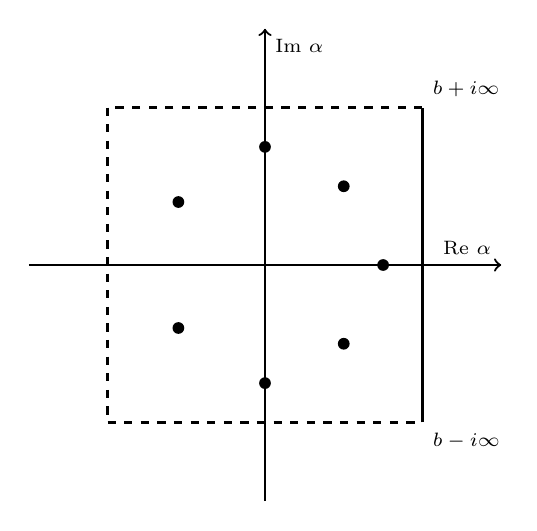
\begin{tikzpicture}
    \begin{scope}[thick,font=\scriptsize]
    % Axes:
    % Are simply drawn using line with the `->` option to make them arrows:
    % The main labels of the axes can be places using `node`s:
    \draw [->] (-3,0) -- (3,0) node [above left]  {Re $\alpha$};
    \draw [->] (0,-3) -- (0,3) node [below right] {Im $\alpha$};

    \draw [-] (2,-2) -- (2,2) node [above right] {$b + i \infty$};
    \draw [dashed] (2,2) -- (-2,2);
    \draw [dashed] (-2,2) -- (-2,-2);
    \draw [dashed] (-2,-2) -- (2,-2) node [below right] {$b - i\infty$};

    %\draw (1,0) node[cross, rotate=45] {};
    \draw (1,1) node[circle, fill, inner sep = 1.5pt] {};
    \draw (1,-1) node[circle, fill, inner sep = 1.5pt] {};
    \draw (-1.1,0.8) node[circle, fill, inner sep = 1.5pt] {};
    \draw (-1.1,-0.8) node[circle, fill, inner sep = 1.5pt] {};
    \draw (1.5,0) node[circle, fill, inner sep = 1.5pt] {};
    \draw (0,1.5) node[circle, fill, inner sep = 1.5pt] {};
    \draw (0,-1.5) node[circle, fill, inner sep = 1.5pt] {};

    \end{scope}
\end{tikzpicture}